% Options for packages loaded elsewhere
\PassOptionsToPackage{unicode}{hyperref}
\PassOptionsToPackage{hyphens}{url}
%
\documentclass[
  12pt,
]{article}
\title{\textbf{State-factor controls on subalpine forest structure}}
\author{Hugh M. Worsham, Energy and Resources Group, U. C.
Berkeley \and Haruko M. Wainwright, Massachusetts Institute of
Technology \and Thomas L. Powell, Sewanee College \and Nicola Falco,
Lawrence Berkeley National Lab \and Lara M. Kueppers, Energy and
Resources Group, U.C. Berkeley, Lawrence Berkeley National Lab}
\date{March 03, 2023}

\usepackage{amsmath,amssymb}
\usepackage[]{mathpazo}
\usepackage{iftex}
\ifPDFTeX
  \usepackage[T1]{fontenc}
  \usepackage[utf8]{inputenc}
  \usepackage{textcomp} % provide euro and other symbols
\else % if luatex or xetex
  \usepackage{unicode-math}
  \defaultfontfeatures{Scale=MatchLowercase}
  \defaultfontfeatures[\rmfamily]{Ligatures=TeX,Scale=1}
\fi
% Use upquote if available, for straight quotes in verbatim environments
\IfFileExists{upquote.sty}{\usepackage{upquote}}{}
\IfFileExists{microtype.sty}{% use microtype if available
  \usepackage[]{microtype}
  \UseMicrotypeSet[protrusion]{basicmath} % disable protrusion for tt fonts
}{}
\usepackage{xcolor}
\IfFileExists{xurl.sty}{\usepackage{xurl}}{} % add URL line breaks if available
\IfFileExists{bookmark.sty}{\usepackage{bookmark}}{\usepackage{hyperref}}
\hypersetup{
  pdftitle={State-factor controls on subalpine forest structure},
  pdfauthor={Hugh M. Worsham, Energy and Resources Group, U. C. Berkeley; Haruko M. Wainwright, Massachusetts Institute of Technology; Thomas L. Powell, Sewanee College; Nicola Falco, Lawrence Berkeley National Lab; Lara M. Kueppers, Energy and Resources Group, U.C. Berkeley, Lawrence Berkeley National Lab},
  pdfkeywords={forest structure, subalpine forest, conifer, ecology,
LiDAR, remote sensing, state factor},
  hidelinks,
  pdfcreator={LaTeX via pandoc}}
\urlstyle{same} % disable monospaced font for URLs
\usepackage[margin = 1in]{geometry}
\usepackage{longtable,booktabs,array}
\usepackage{calc} % for calculating minipage widths
% Correct order of tables after \paragraph or \subparagraph
\usepackage{etoolbox}
\makeatletter
\patchcmd\longtable{\par}{\if@noskipsec\mbox{}\fi\par}{}{}
\makeatother
% Allow footnotes in longtable head/foot
\IfFileExists{footnotehyper.sty}{\usepackage{footnotehyper}}{\usepackage{footnote}}
\makesavenoteenv{longtable}
\usepackage{graphicx}
\makeatletter
\def\maxwidth{\ifdim\Gin@nat@width>\linewidth\linewidth\else\Gin@nat@width\fi}
\def\maxheight{\ifdim\Gin@nat@height>\textheight\textheight\else\Gin@nat@height\fi}
\makeatother
% Scale images if necessary, so that they will not overflow the page
% margins by default, and it is still possible to overwrite the defaults
% using explicit options in \includegraphics[width, height, ...]{}
\setkeys{Gin}{width=\maxwidth,height=\maxheight,keepaspectratio}
% Set default figure placement to htbp
\makeatletter
\def\fps@figure{htbp}
\makeatother
\setlength{\emergencystretch}{3em} % prevent overfull lines
\providecommand{\tightlist}{%
  \setlength{\itemsep}{0pt}\setlength{\parskip}{0pt}}
\setcounter{secnumdepth}{-\maxdimen} % remove section numbering
\newlength{\cslhangindent}
\setlength{\cslhangindent}{1.5em}
\newlength{\csllabelwidth}
\setlength{\csllabelwidth}{3em}
\newlength{\cslentryspacingunit} % times entry-spacing
\setlength{\cslentryspacingunit}{\parskip}
\newenvironment{CSLReferences}[2] % #1 hanging-ident, #2 entry spacing
 {% don't indent paragraphs
  \setlength{\parindent}{0pt}
  % turn on hanging indent if param 1 is 1
  \ifodd #1
  \let\oldpar\par
  \def\par{\hangindent=\cslhangindent\oldpar}
  \fi
  % set entry spacing
  \setlength{\parskip}{#2\cslentryspacingunit}
 }%
 {}
\usepackage{calc}
\newcommand{\CSLBlock}[1]{#1\hfill\break}
\newcommand{\CSLLeftMargin}[1]{\parbox[t]{\csllabelwidth}{#1}}
\newcommand{\CSLRightInline}[1]{\parbox[t]{\linewidth - \csllabelwidth}{#1}\break}
\newcommand{\CSLIndent}[1]{\hspace{\cslhangindent}#1}
\usepackage{setspace}\doublespacing
\usepackage[left]{lineno}
\usepackage{indentfirst}
\setlength\parindent{24pt}
\linenumbers
\usepackage{dcolumn}
\usepackage{caption}
\usepackage{float}
\usepackage{afterpage}
\usepackage{siunitx}
\usepackage{amsmath}
\ifLuaTeX
  \usepackage{selnolig}  % disable illegal ligatures
\fi

\begin{document}
\maketitle
\begin{abstract}
Abstract goes here.
\end{abstract}

\hypertarget{introduction}{%
\section{Introduction}\label{introduction}}

One strain of thinking in ecology holds that ecosystem development is a
function of five state factors: topography, parent material, climate,
organisms, and time (Amundson and Jenny, 1997; Jenny, 1961). Forest
stand structure and composition are two emergent properties of ecosystem
development that can be evaluated in terms of continuous variables
observed at a given point in time. Quantifying the relationships between
an ecosystem's structure and composition and its underlying state
factors is a fundamental concern for ecology and biochemistry
{[}Vitousek and Matson 1991 {[}TODO: fix cite{]}{]}. While general
relationships are acknowledged between (on the one hand) topographic,
edaphic, lithologic, and climate state variables and (on the other)
mature forest structure and composition, few studies have quantified the
relative importance of state factors to stand structure and composition,
or their potential interactive effects, particularly in subalpine
domains. Several studies of the spatial variability of stand density,
size distribution, and species composition in montane and subalpine
forests have produced inconsistent results {[}e.g.~Underwood et
al.~2010; Lydersen and North (2012, TODO: other citations){]}. These
inconsistencies suggest that at least some inferences about these
relationships reflect an insufficient reckoning of how state factors
interact to affect the hydrologic and energetic conditions in which
plants grow (Lookingbill and Urban, 2004). Moreover, only a handful of
papers have used spatially continuous estimates of stand structure to
capture the full range of variability in either state factors or
emergent ecosystem properties. This has been especially difficult to
achieve in high-elevation, mountainous terrain because end-members on
topographic and climate gradients are often inaccessible for field
measurement. This limitation may now be partially overcome with active
remote sensing technologies, such as light detection and ranging (LiDAR)
({[}TODO: cite{]}). Because biogeochemical fluxes between forests and
the atmosphere are influenced by stand structure and composition,
measuring these characteristics and their underlying environmental
drivers is a central objective for forest ecology, conservation, and
management {[}Waring and Running 1998{]}.

\hypertarget{variability-in-forest-structure-and-composition}{%
\subsection{Variability in forest structure and
composition}\label{variability-in-forest-structure-and-composition}}

\hypertarget{forest-structure-and-topography}{%
\subsubsection{1. Forest structure and
topography}\label{forest-structure-and-topography}}

Topographic properties such as elevation, slope, hillslope position,
curvature, and aspect substantially influence local microclimate and
soil moisture variability {[}Dobrowski 2011{]}. As a result, they
directly and indirectly constrain trees' growing environments,
influencing demographic rates and exposure to disturbance, and
ultimately shaping stand structure, composition, and function (Kane et
al., 2015). Even in low-diversity forests, physiognomy can vary
dramatically with small changes in position. This variability is often
especially pronounced in mountainous terrain, owing to the potential for
large changes in elevation, slope, and aspect over small horizontal
distances {[}Dobrowski 2011{]}.

In complex terrain, pronounced gradients of insolation, precipitation
input, and subsurface water distribution influence plant demographic
processes, including productivity, biomass accumulation, and recruitment
and mortality. Topography can also influence disturbance frequency and
magnitude, drought and temperature stress, wind exposure, in turn
influencing biotic structure and composition. General trends are assumed
(McNab, 1993, 1989), \emph{but quantitative reporting is limited in the
literature} {[}TODO: verify{]}. In general, topographic factors can be
important determinants of forest structure and composition, and
elevation, aspect, and position on the hillslope matter most. Stem
diameter, basal, area, and growth rates decline with elevation, with
temperature as the key limiting control. The same properties also
decline from valley to ridge positions, and from polar to equatorial
exposures, perhaps as a result of these factors' influence on soil
moisture and vapor pressure deficit (Bolstad et al., 2018; McNab, 1993,
1989).

While these patterns may describe general relationships, there is
evidence that they can vary in both magnitude and direction across
watersheds and landscapes {[}Kelsey et al.~2018 {[}TODO: fix cite{]}{]}.
Lydersen and North (2012) reported contrary findings in a Sierra Nevada
mixed conifer forest, where upper slopes had both the highest quadratic
mean diameter (QMD) and the tallest trees. Kane et al. (2015),
furthermore, found that topography explained little variance in forest
structure in a domain with a frequent fire return interval.

\hypertarget{forest-composition-and-topography}{%
\subsubsection{2. Forest composition and
topography}\label{forest-composition-and-topography}}

Topography may also exert control on species mix {[}Rowe and Sheard
1981; Barnes et al.~1982; Bailey 1988 {[}TODO: fix cites{]}{]}. Species
affinities for certain topographic positions may be attributable to
functional strategies developed in response to variability in radiative
(Monin et al.~2007; White and Millet 2008) and hydrologic {[}Whittaker
1956, Day and Monk 1988; Hawthorne and Miniaat 2018 {[}TODO: fix
cites{]}{]} regimes. In subalpine forests of the southern Rocky
Mountains (SRM), some clear topography-driven controls on species
occurrence exist. Engelmann spruce (\emph{Picea engelmannii}) and
subalpine fir (\emph{Abies lasiocarpa}) tend to co-occur in high
densities throughout the subalpine zone (\textasciitilde2700---3000 m
a.s.l.) and only sparsely in the upper montane zone
(\textasciitilde1850--2900 m a.s.l.). At middle and high elevations up
to treeline, the longer-lived spruce is often the canopy dominant
(\textasciitilde70 percent of canopy basal area), while fir may occupy
up to the same proportion of the understory (Alexander et al.~1984).
Near treeline, pure spruce stands are common, while fir often dominate
the canopy in the lower end of the subalpine zone, particularly in xeric
topographic positions (Alexander 1987). Douglas fir (\emph{Pseudotsuga
menziesii}) tend to dominate mesic sites, including north-facing
toe-slopes and high-elevation south-facing slopes. Lodgepole pine
(\emph{Pinus contorta}) also occurs on dry, southerly upper slopes in
the lower range of the subalpine zone, and abundantly throughout the
montane zone, particularly on south-facing slopes and steep slopes of
all aspects (Veblen 1986).

\hypertarget{forest-structure-and-soil}{%
\subsubsection{3. Forest structure and
soil}\label{forest-structure-and-soil}}

Soil properties also matter for structural development. Parent material
in the top 10 cm of soil explained a greater share of variation in the
abundance of trees across global biomes than any other single factor,
including climate and topography (Delgado-Baquerizo et al.~2020). Parent
material is also a significant explainer of ecosystem productivity.
{[}TODO: more on soil and forest structure from conifer forests in
montane, subalpine zones{]}.

\hypertarget{forest-composition-and-soil}{%
\subsubsection{4. Forest composition and
soil}\label{forest-composition-and-soil}}

{[}TODO: more on soils from conifer forests in montane, subalpine zones,
focusing on soil composition, available water capacity, organic
matter{]}

\hypertarget{forest-structure-composition-and-climate}{%
\subsubsection{5. Forest structure, composition, and
climate}\label{forest-structure-composition-and-climate}}

In forest ecosystems, gradient analysis has consistently identified
temperature and water balance as the strongest abiotic factors
explaining vegetation species distributions and emergent properties such
as canopy structure and carbon density (Veblen 1986, Urban et al.~2000,
Hessberg et al.~2007, Holden and Jolly 2011). Elevation-driven lapse
rate is assumed to exert the strongest control on tree growth and
stature, as well as biomass accummulation. Conifer height tends to
decline with temperature and with precipitation (Swensen and Weiser,
Hulshof et al.~2015). Yet, temperature and precipitation can be
extremely heterogeneous in mountain domains with high topographic
relief, and do not uniformly track elevation. A site's temperature and
radiation regimes may be further regulated by exposure angle and shading
by adjacent landforms, while its precipitation regime may be regulated
by orogenic cloud formation, which can decouple local precipitation
patterns from regional patterns {[}TODO: cite{]}. Moreover, variability
in wind exposure leads to snow redistribution, yielding patterns of
accumulation and melt that may differ from snowfall patterns ({[}TODO:
citation, see ASO, Deems et al.{]}). {[}TODO: more on compositional
relationships with climate{]}.

\hypertarget{gaps-and-motivations}{%
\subsection{Gaps and motivations}\label{gaps-and-motivations}}

The majority of gradient analyses use elevation, convergence, or
landscape position as proxies for temperature and soil moisture
(Stephenson 1998; Ng et al.~2020). A smaller subset of studies have
deployed more complex metrics that combine factors such as elevation,
hillslope position, aspect, and slope into quasi-independent
climate-proxy variables. Urban and colleagues (2000) used elevation,
slope aspect, topographic convergence, and soil depth to model a
``physical template'' describing the light, temperature, and soil
moisture regime of a Sierra Nevada domain, and then examined the
sensitivity of model-estimated forest stand basal area, fuel loading,
and canopy depth to the topographic inputs. Underwood and colleagues
(2010) used elevation, slope, aspect, solar radiation, and topographic
wetness to divide a Sierra Nevada domain into ``landscape management
units'' representing nine clusters of topographic variability, and
examined variation in stem and species density across those units. Their
effort relied on data collected \emph{in situ} from 164 transects.

First, while plot- and transect-based data can provide reliable
estimates of aboveground forest structure and composition when scaled up
to a stand, these data are by nature limited in spatial extent and do
not represent the full range of state-factor variability that may
constrain the distribution of vegetation across a landscape (Hurtt et
al.~2004, Antonarakis et al.~2011, Lydersen and North (2012),
Antonarakis et al.~2014). Even within mature, close-canopied forests,
characteristics such as stand density, age-class distribution,
allometry, species composition, and species dominance can have wide
variance. Efforts to scale these properties up to a watershed from plot
observations (or plot-benchmarked models) alone can yield substantial
error terms. Therefore, prior work may have failed to capture important
dimensions of co-variability. Kane et al.~(2015) and Bolstad et
al.~(2018) are the only studies we have identified that evaluate
spatially continuous measures of topography and forest structure,
although more results have been reported from tropical forests
(e.g.~Chadwick and Asner 2015, Jucker et al.~2018).

A further concern is that the statistical modeling strategies used in
prior studies are unable to quantify potential interactions among
topographic variables. Factors such as elevation, hillslope, and
curvature work together to define a site's edaphic, radiative, and
moisture environments. Failing to account for these interactions may
amount to a significant oversight. In part because of these limitations,
ecology still lacks a complete accounting of how forest physiognomy
co-varies with state factors.

LiDAR integrated with field sampling {[}and hyperspectral remote
sensing{]} holds promise for overcoming some of these limitations.
Advances in active remote sensing, including in light detection and
ranging (LiDAR), have opened up new opportunities for characterizing
forest structure on a continuous basis for a wide array of scientific
and management applications (Mallet and Bretar 2009). In particular,
over the past five years a profusion of full waveform LiDAR datasets
from aerial and satellite platforms, and emerging open-source libraries
for cleaning and processing the data, has enabled more accurate
estimates of forest structure than those from discrete-return
acquisitions (Zhou and Popescu 2017). Like discrete-return points,
waveform data can be used to delineate individual canopy trees and to
estimate individual-scale characteristics such as stem diameter, stem
height, stem volume, and crown volume (Dalponte et al.~2011, Jucker et
al.~2017). Waveforms can also be processed to generate continuous
estimates of forest structure parameters at the pixel-grid scale; these
parameters include aboveground biomass, leaf-area index, total number
density, and diameter-class distribution. While some researchers have
eschewed individual tree object--based approaches because of the
difficulty of characterizing subcanopy structure with dicrete-return
data, a profusion of new algorithms aimed at waveform and hyper-dense
point clouds has made it increasingly possible to achieve
individual-based structure estimates. Using the full waveforms appears
to improve the accuracy of both object-oriented and continuous-estimate
methods over discrete-return estimates, particularly for characterizing
mid-canopy and sub-canopy structure. Integrating waveforms with imaging
spectrometry and calibrating remote sensing against \emph{in situ} stem
diameter and height measurements yields further accuracy improvements
(Antonarakis et al.~2011, Jucker et al.~2017).

Quantifying the drivers of fine-scale heterogeneity in the structure,
composition, and function of montane and subalpine forests is important
for several reasons. First, understanding the factors that shape
landscape vegetation patterns remains a foundational question in ecology
and conservation (Waring and Running 1998, Turner and Gardner 2015).
Second, as in most systems that face the imminent prospect of novel
drought and disturbance regimes, there is a need for reference data
against which scientists and managers can observe change (Millar et
al.~2007). Third, understanding the drivers of heterogeneity is
essential for forecasting how mountain forests will respond to regional
environmental change, and for devising conservation and management
strategies that promote forest resilience. Finally, there is a need for
both data and inferential analyses that can be used to initialize and
benchmark terrestrial ecosystem models used to predict vegetation and
flux responses to perturbations (Antonarakis et al.~2011, Antonarakis et
al.~2014)

While previous studies have identified general state-factor responses in
forest structure and composition, to our knowledge, no study accounts
for topographic, edaphic, lithologic, and climate influences on multiple
stand structural and compositional properties together. Few studies
directly address microclimatic heterogeneity in high-elevation complex
terrain, and none account for state-variable interactions. None does the
above on a spatially continuous basis, incorporating end-members on the
radiative and moisture gradients along which forest stands grow.

Our primary objective in this study was to quantify relationships
between forest structure/composition and environmental attributes
representing the main state factors that drive stand structural
development in subalpine forests broadly representative of low-diversity
forests across the Southern Rocky Mountains.

We addressed the following questions:

\begin{enumerate}
\def\labelenumi{\arabic{enumi}.}
\tightlist
\item
  To what extent are tree stem height and diameter distributions, total
  number density, and basal area influenced by the elevation, slope,
  hillslope position, solar radiation, aspect, and topographic wetness
  of a site?
\item
  To what extent are species distributions influenced by the same
  topographic factors?
\item
  How do the specified topographic factors interact to mediate these
  relationships?
\end{enumerate}

To address these questions, we integrated a full-waveform LiDAR dataset
acquired over Colorado's East River watershed with {[}a species
classification map derived from imaging spectrometry and{]} field
inventory measurements of 7000+ trees to quantify the spatial
variability of forest canopy structure through the vertical profile, as
well as stand structure and composition. We then used inferential
modeling techniques to quantify the relative importance of state-factor
controls on forest stand structure and composition, as estimated at a
single point and time.

\hypertarget{data-and-methods}{%
\section{Data and methods}\label{data-and-methods}}

\hypertarget{a.-study-area}{%
\subsection{A. Study area}\label{a.-study-area}}

The domain for this project comprised montane-subalpine conifer forest
stands in Colorado's East River watershed (38°55' N, 106°56' W; Fig. 1).
The East River is a headwater tributary of the Colorado River, the
principal freshwater source for one in 10 people in the U.S. (U.S.
Department of the Interior Bureau of Reclamation 2012). The
\textasciitilde750 \(km^2\) catchment includes six major drainages with
perennial snowmelt-fed streams. It also has significant topographic
heterogeneity: 1420 m of elevational relief, multiple peaks extending
above treeline, and pronounced gradients in slope, aspect, insolation,
and hillslope position. Mean annual temperature measured at a SNOTEL
site (736-Schofield) at 3261 m in the northern reach of the watershed is
1.8 º C, with maximum and minimum of 8.3 º C and --28.4 º C
respectively. Mean annual precipitation is \textasciitilde1200 mm
\(y^{–1}\), approximately 70 percent as snow and 30 percent as rain.
Maximum air temperatures are depressed by wind at high elevations and
minimum air temperatures by cold air downwelling at low elevations.
Precipitation is also strongly influenced by elevation, with snow
accumulation generally increasing upgradient. The system is driven by
seasonal temperature and precipitation regimes that impose important
controls on vegetation phenology. Winter snows arrive as early as
September, and storms may persist into early June at the highest
elevations. Snowmelt typically begins in April and continues through
June, concurrently with initiation of vegetation growth {[}TODO:
confirm; growth may start up before melt{]}. A seasonal drydown occurs
in late June and July, characterized by sparse rainfall and soil
desiccation as evaporative demand rises with summer temperatures (Harte
et al.~1995). In most years, this seasonal moisture deficit is partially
mitigated by a July--August monsoon. The driest phase occurs over
August--September and can drive severe soil moisture deficits in years
when the monsoon fails, as it did in 2018. In addition to these broad
patterns, the domain's stark relief and topographic complexity
coordinate to produce highly variable local climatic conditions.Soils
are derived from varied, primarily sedimentary material intruded by
igneous laccoliths. Mancos Shale is the dominant bedrock. Heterogeneous
soil composition and drainage potential drives substantial variability
in plant available water. The domain spans montane to alpine ecosystems
(2700 m to 3500 m). The dominant tree species are \emph{P. engelmannii},
\emph{A. lasiocarpa}, \emph{P. contorta}, and \emph{Populus
tremuloides}, with occasional \emph{P. menziesii} at mid-elevations and
one known population of \emph{Pinus longaeva} near treeline on one
summit.

\hypertarget{b.-data-summary}{%
\subsection{B. Data summary}\label{b.-data-summary}}

Primary data included field census data from 17 permanent mixed-conifer
inventory plots, each 0.16 ha in area; a June 2018 National Ecological
Observatory Network Airborne Observation Platform (NEON AOP) full
waveform LiDAR acquisition; a species-level classification map developed
form a simultaneous NEON hyperspectral acquisition (Falco et al.~2022);
a digital elevation model (DEM) interpolated from NEON LiDAR ground
return points.

\hypertarget{c.-data-collection-and-processing}{%
\subsection{C. Data collection and
processing}\label{c.-data-collection-and-processing}}

\hypertarget{field-census}{%
\subsubsection{1. Field census}\label{field-census}}

Between 2018 and 2022, we established 25 long-term forest monitoring
plots around the East River and nearby drainages. The sites were
stratified across six topographic gradients. An initial set of 68 sites
was preselected via Latin hypercube sampling on six topographic
gradients derived from the USGS 1/3-arc second digital elevation model
(DEM) {[}TODO: cite{]}. The gradients are described in Table 1. The
distribution of plots along those gradients and correlation statistics
for topographic variable pairs appear in Appendix A. The final 25 sites
were selected from among that group after scouting and optimizing the
distribution of the set along the topographic gradients.

We installed square 40x40 m plots by staking one corner and running a
metric tape in a straight line to a point 40 m away to form one edge of
the plot. The cardinal orientation and slope angle between points were
measured with a digital compass and laser hypsometer, respectively, and
the approximate location of the next corner was sighted at an angle of
90º and distance of 40 m from the first. A second tape was run to the
approximate corner, and adjusted to achieve the exact distance and
angle. This process was repeated for the four edges. The cardinal
orientation and slope angle between corners were then remeasured and the
distance between corners was adjusted using trigonometric corrections,
to approximate a projected flat-surface area of 1600 m.

We conducted a field census of approximately 9000 trees in the 25 plots.
All trees of any species with a diameter at breast height (DBH, measured
at 1.3 m) \textgreater1.0 cm were tagged with an aluminum tag affixed
with a nail if the specimen was \textgreater10cm DBH and with an
expanding collar if the specimen was \textless10cm DBH. Measurements
taken from each tree are summarized in Table 2.

Seventeen of the 25 plots lay within the overflight footprint of a 2018
NEON AOP acquisition (Kampe et al.~2009). We used the observations from
this subset for training and validation of models developed in the next
phase of analysis. This set comprised 6700 {[}TODO: confirm{]} trees.

\hypertarget{waveform-lidar-processing}{%
\subsubsection{2. Waveform LiDAR
processing}\label{waveform-lidar-processing}}

Between June 12 and 26, 2018, the NEON AOP surveyed approximately
\(330 km^2\) of the watershed (Chadwick et al.~2020; Fig. 1). The AOP
collected LiDAR using an Optech Gemini discrete LiDAR sensor and
waveform digitizer. The LiDAR sensor's pulse repetition frequency varied
between 33 and 100 kHz. The platform also collected high-fidelity VSWIR
spectrometry at 1 m resolution using an AVRIS-NG visible and infrared
imaging spectrometer. The spectrometer and LiDAR platforms were
co-aligned with an onboard GPS/IMU system. Validation was conducted
using in situ data at 437 sites representing a range of vegetative and
built land cover types.

Discrete-return point density in the post-processed dataset ranged
between 1 and 9 returns \(m^{-2}\), which was insufficient for
characterizing subcanopy structure. We therefore elected to analyze the
full waveforms, which had a nominal density between 1 and 4 pulses
\(m^{-2}\). We were able to exploit the higher information-density of
full-waveform pulses to develop more complete characterizations of stand
and canopy structure than would have been possible with discrete returns
alone.

\hypertarget{waveform-processing}{%
\subsubsection{3. Waveform processing}\label{waveform-processing}}

We generated both an individual tree crown (ITC) map and continuous
gridded estimates of mixed-conifer forest structure (as in Dalponte and
Coomes (2016)). The former comprises a map of individual tree crowns in
mixed-conifer forest stands describing species, height, crown area, and
stem diameter of each tree, along with estimates of detection error. The
latter comprises a continuous map of forest structure metrics at 10m,
40m, 100m, and 1km grid scales. We pursued the following steps to
produce these datasets.

First, we used a spectral deconvolution procedure to isolate the
target-response signal from its interactions with the LiDAR system's
outgoing pulse, atmospheric scattering, and sensor-system noise. We used
the Gold deconvolution algorithm contained in Zhou et al.'s (2017)
implementation in the \texttt{waveformlidar} package in the R
statistical computing environment, but refactored their implementation
for parallel computing. The result of the algorithm approximates the
true distribution of scattering objects along the outbound light pulse's
path.

The signal intensity of an outbound LiDAR pulse as a function of time is
roughly Gaussian in shape. As the pulse interacts with physical objects
along its path and is reflected back to the sensor, the returning
backscatter cross-section can also be expressed approximately as a sum
of Gaussian functions. Gaussian decomposition allows one to characterize
the components of the returning impulse (Harding 2005). We applied an
adaptive Gaussian decomposition procedure to fit one or more Gaussian
models to each return pulse based on Equation 2:

\[f(x,\theta) = \sum_{(i=1)}^{n} A_i exp\biggl[-\frac{(x-\mu_i)^\lambda}{(2\sigma_i^2)}\biggr]\]
(2) where \(A_i\) is the amplitude of waveform component \(i\), \(\mu\)
is the bin location of \(i\) (measured as a point in time, ns),
\(\sigma\) is the standard deviation of \(i\), and \(\lambda\) is a
penalty parameter that minimizes model residual over a specified number
of iterations. The algorithm first identifies potential peaks in the
waveform, then iteratively fits a model to each peak. It then selects
the model that minimizes root mean square error between the raw waveform
and fitted values, excluding models that produce physically meaningless
parameters (such as a negative \(A_i\)). Where multiple peaks exist, the
algorithm fits a separate function to each and expresses the final fit
as the sum of n Gaussian functions. Fitting was accomplished using the
\texttt{nlsLM} in the R package \texttt{minpack.lm}.

The deconvolution and decomposition procedures were applied to the full
set of waveforms (\textasciitilde500 x 4e9) {[}TODO:confirm dim{]} in
parallel on 256 cores on the University of California, Berkeley's
high-performance computing cluster.

After processing the waveforms, we used the geolocation matrices
provided in the NEON dataset to geolocate the waveforms and extracted
characteristic metrics from the fitted waveforms. These included the
peaks' location in three-dimensional space, their amplitude and width,
front slope, and time to median intensity. We then used the R package
\texttt{lidR} to discretize this information along with the geolocated
waveform data. We normalized the discretized points to the earth surface
by differencing their z-values against a DEM derived from the
discrete-return point cloud included in the NEON dataset (Fig. 3). We
then decimated the high-density returns, preserving all of the
identified Gaussian peaks and randomly sampling non-peak intensities to
obtain a point cloud with a uniform density of 16--18 points
\(m^{2^-1}\) across the full domain.

\hypertarget{tree-segmentation-and-cross-validation}{%
\subsubsection{4. Tree segmentation and
cross-validation}\label{tree-segmentation-and-cross-validation}}

Next, we integrated the processed LiDAR data and field data from
inventory plots to train and validate an individual tree delineation
(ITD) model, which we then applied to the remaining forested area to
generate a tree crown map of the watershed. We used a leave-one-out
cross-validation (LOOCV) strategy to optimize tree crown delineation at
the field sites. This approach iterated through a range of possible
parameters for each of seven ITD algorithms, then selected the
best-performing algorithm and parameter set to apply to the remaining
data.

First, we extracted the discretized waveform data intersecting the
boundaries of each field plot plus a 10 m buffer on all sides. At each
step of cross-validation we randomly removed one plot from
consideration, then attempted tree segmentation on the point data in the
remaining 16 plots using algorithm \(A_i\) and parameter set
\(\lambda_{i,j:k}\), where \(i\) is the \(i\)th algorithm and \(j:k\)
are vectors of values on the parameters required for the algorithm to
proceed. In each run we linked delineated trees to their nearest
field-observed trees by matching nearest neighbors in the Euclidean
space described by the latitude-longitude-height coordinates of modeled
stems and the latitude-longitude-height coordinates of stems geotagged
in the field. We then computed the loss between model and observation as

\[ loss_{i,j} = \frac{\sum_{i,j=1}^{n}\sqrt{(x_i-x_j)^2+(y_i-y_j)^2+(z_i-z_j)^2}}{p(match)}\]
where \(i\) is the \(i\)th modeled tree and \(j\) is its linked
field-observed tree; \(x\), \(y\), and \(z\) are the longitude,
latitude, and height coordinates of \(i\) and \(j\), respectively, and
\(p(match)\) is the ratio of successfully matched trees to
field-observed trees. This loss term is effectively the sum of Euclidean
distances between pairs of matched tree summits penalized by poor match
rates. For each run of \(\lambda_{i,j:k}\) on \(A_i\) we stored the
computed loss, then selected the parameter combination corresponding to
the minimum loss value across all \(\lambda_{i,j:k}\). We used this
parameter combination to delineate trees in the held-out plot, and
computed the loss on this test set. We repeated this procedure until we
had cycled through all LOOCV permutations, and averaged the 17 test loss
scores. Each of these steps was then implemented for the next algorithm
\(A_{i}\). We ran this operation with seven ITD algorithms (described in
Appendix B) and a total of {[}TODO: confirm number{]} of parameters, and
selected the algorithm and parameter set that yielded the minimum
average loss.

For the remainder of the LiDAR-surveyed domain, we subset the
discretized waveforms over conifer forest by finding their intersection
with conifer-classified areas from a land-cover classification map
derived from the NEON hyperspectral acquisition (Breckheimer 2021). We
forced the optimal algorithm with this subset of LiDAR data and the
optimal parameter set from training to delineate all tree crowns in the
watershed's conifer stands. The result was a spatially continuous
dataset of conifer tree objects describing their locations, heights, and
estimated crown areas. To estimate the stem diameters of each delineated
object, we used an allometric function of stem height with coefficients
derived from plot observations. {[}TODO: write functional form{]}.

{[}TODO: Implement this part or cut if it doesn't pan out: The
tree-crown product was fused with a 1 m resolution forest species
classification dataset, developed through a support vector machine
classifier on 2018 NEON AOP hyperspectral imagery (Falco 2020). Each
object was assigned to a given tree species according to the majority
rule, i.e., if 50 percent or more of the pixels intersecting the object
were classified to that species (Dalponte et al.~2019). For trees where
less than 50 percent of pixels belonged to a single species, the object
was labeled ``unknown.''{]}

From the fused dataset, we computed continuous area-based structural
{[}and compositional{]} metrics by summarizing object-level predictions
at specified grid scales across the watershed. Structural metrics
included total number density, basal area, quadratic mean diameter, and
diameter and height percentiles. {[}TODO: Compositional metrics included
species composition (proportion of pixel area occupied by each species),
species density (number of individuals of each species per pixel), and
species dominance (majority species per pixel).

\hypertarget{inferential-modeling}{%
\paragraph{5. Inferential modeling}\label{inferential-modeling}}

The final phase of the analysis evaluated the relationships between
these structural {[}and compositional{]} metrics to spatially continuous
estimates of underlying state factors. I will use these structure and
composition data layers along with topographic features derived from a
digital elevation model, all at 100m resolution, to evaluate the effects
of topographic position on species composition and forest structure. The
explanatory and response variables are summarized in Table 3.

\hypertarget{results}{%
\section{Results}\label{results}}

\hypertarget{subresults-1}{%
\subsection{Subresults 1}\label{subresults-1}}

\hypertarget{subresults-2}{%
\subsection{Subresults 2}\label{subresults-2}}

\hypertarget{discussion}{%
\section{Discussion}\label{discussion}}

\hypertarget{conclusions}{%
\subsection{Conclusions}\label{conclusions}}

\hypertarget{acknowledgements}{%
\section{Acknowledgements}\label{acknowledgements}}

\clearpage

\newpage

\hypertarget{figures-and-tables}{%
\section{Figures and Tables}\label{figures-and-tables}}

\hypertarget{figure-1}{%
\subsection{Figure 1}\label{figure-1}}

\includegraphics{./Figures/Fig1.png} \textbf{Figure 1.} The study domain
spans the footprint of a June 2018 NEON AOP acquisition in the East
River watershed in western Colorado. Dots indicate the locations of 0.16
ha conifer forest inventory plots. Shading is by elevation. \clearpage

\newpage

\hypertarget{table-1}{%
\subsection{Table 1}\label{table-1}}

\textbf{Table 1.} Description and units of topographic variables used
for field plot selection.

\begin{longtable}[]{@{}
  >{\raggedright\arraybackslash}p{(\columnwidth - 4\tabcolsep) * \real{0.33}}
  >{\raggedright\arraybackslash}p{(\columnwidth - 4\tabcolsep) * \real{0.46}}
  >{\raggedright\arraybackslash}p{(\columnwidth - 4\tabcolsep) * \real{0.21}}@{}}
\toprule
\begin{minipage}[b]{\linewidth}\raggedright
Variable
\end{minipage} & \begin{minipage}[b]{\linewidth}\raggedright
Description
\end{minipage} & \begin{minipage}[b]{\linewidth}\raggedright
Units
\end{minipage} \\
\midrule
\endhead
Elevation & Elevation above sea level & m \\
Slope & dy/dx computed in a 30 m window & degrees \\
Folded aspect & Index of cardinal aspect adjusted for higher incident
radiation on SW slopes & unitless index \\
Heat load & Potential heat load calculated according to Eq. 3 in McCune
and Keon (2002) & unitless index \\
Topographic position index (1000 m) & Index of hillslope position
(summit, shoulder, backslope, footslope, and toeslope) computed in 1000
m window & unitless index \\
Topographic wetness index & Terrain-driven balance of upslope water
supply and local drainage (a function of local slope and upslope
contributing area per unit contour length) & unitless index \\
\bottomrule
\end{longtable}

\clearpage

\newpage

\hypertarget{table-2}{%
\subsection{Table 2}\label{table-2}}

\textbf{Table 2.} Measurements taken in field inventory with their units
and a summary of methods.

\begin{longtable}[]{@{}
  >{\raggedright\arraybackslash}p{(\columnwidth - 4\tabcolsep) * \real{0.50}}
  >{\raggedright\arraybackslash}p{(\columnwidth - 4\tabcolsep) * \real{0.23}}
  >{\raggedright\arraybackslash}p{(\columnwidth - 4\tabcolsep) * \real{0.27}}@{}}
\toprule
\begin{minipage}[b]{\linewidth}\raggedright
Measurement
\end{minipage} & \begin{minipage}[b]{\linewidth}\raggedright
Units
\end{minipage} & \begin{minipage}[b]{\linewidth}\raggedright
Method
\end{minipage} \\
\midrule
\endhead
Species & NA & Visual identification \\
Stem height & m & Nikon Forestry Pro II hypsometer, metric tape \\
DBH & cm & Diameter tape, calipers \\
Stem geolocation & decimal degrees & Trimble GEO-7X GPS unit held
against stem \\
Crown illumination & unitless index & Visual determination \\
Beetle damage & unitless index & Visual inspection for boreholes, sap,
red/grey needles \\
Life status & NA & Visual inspection for living/dead status \\
Health status & NA & Visual inspection for signs of infection, decay,
browning, wilting \\
\bottomrule
\end{longtable}

\clearpage

\newpage

\hypertarget{figure-2}{%
\subsection{Figure 2}\label{figure-2}}

\includegraphics{./Figures/Fig2.png} \textbf{Figure 2.} Diameter and
height distributions of trees measured in inventory plots across all
sites (A), and by species (B, C). \clearpage

\newpage

\hypertarget{figure-3}{%
\subsection{Figure 3}\label{figure-3}}

\includegraphics{./Figures/Fig3.png} \textbf{Figure 3.} Raw waveforms
were deconvolved with the outgoing ALS pulse and instrument impulse
response using the Gold algorithm, and then decomposed into a sum of
fitted Gaussian functions over time. Panel A shows the raw (dashed
black) waveform function and the resulting deconvolved (dark blue) and
decomposed (light blue) time series, all over a trimmed 100 ns support.
Waveform peaks and a random sample of values along peak slopes were
selected to generate a point cloud with a mean density of 24 points m2-1
across the acquisition area. An example of this high-density point cloud
at one inventory plot (SG-SWR1) with a 10 m buffer is shown in panel B.
The result of individual tree segmentation at the same plot, with buffer
removed, appears in panel C. \clearpage

\newpage

\hypertarget{figure-4}{%
\subsection{Figure 4}\label{figure-4}}

\includegraphics{./Figures/Fig4.png} \textbf{Figure 4.} Maps of forest
structure metrics at 100 m grid resolution. \clearpage

\newpage

\hypertarget{figure-5}{%
\subsection{Figure 5}\label{figure-5}}

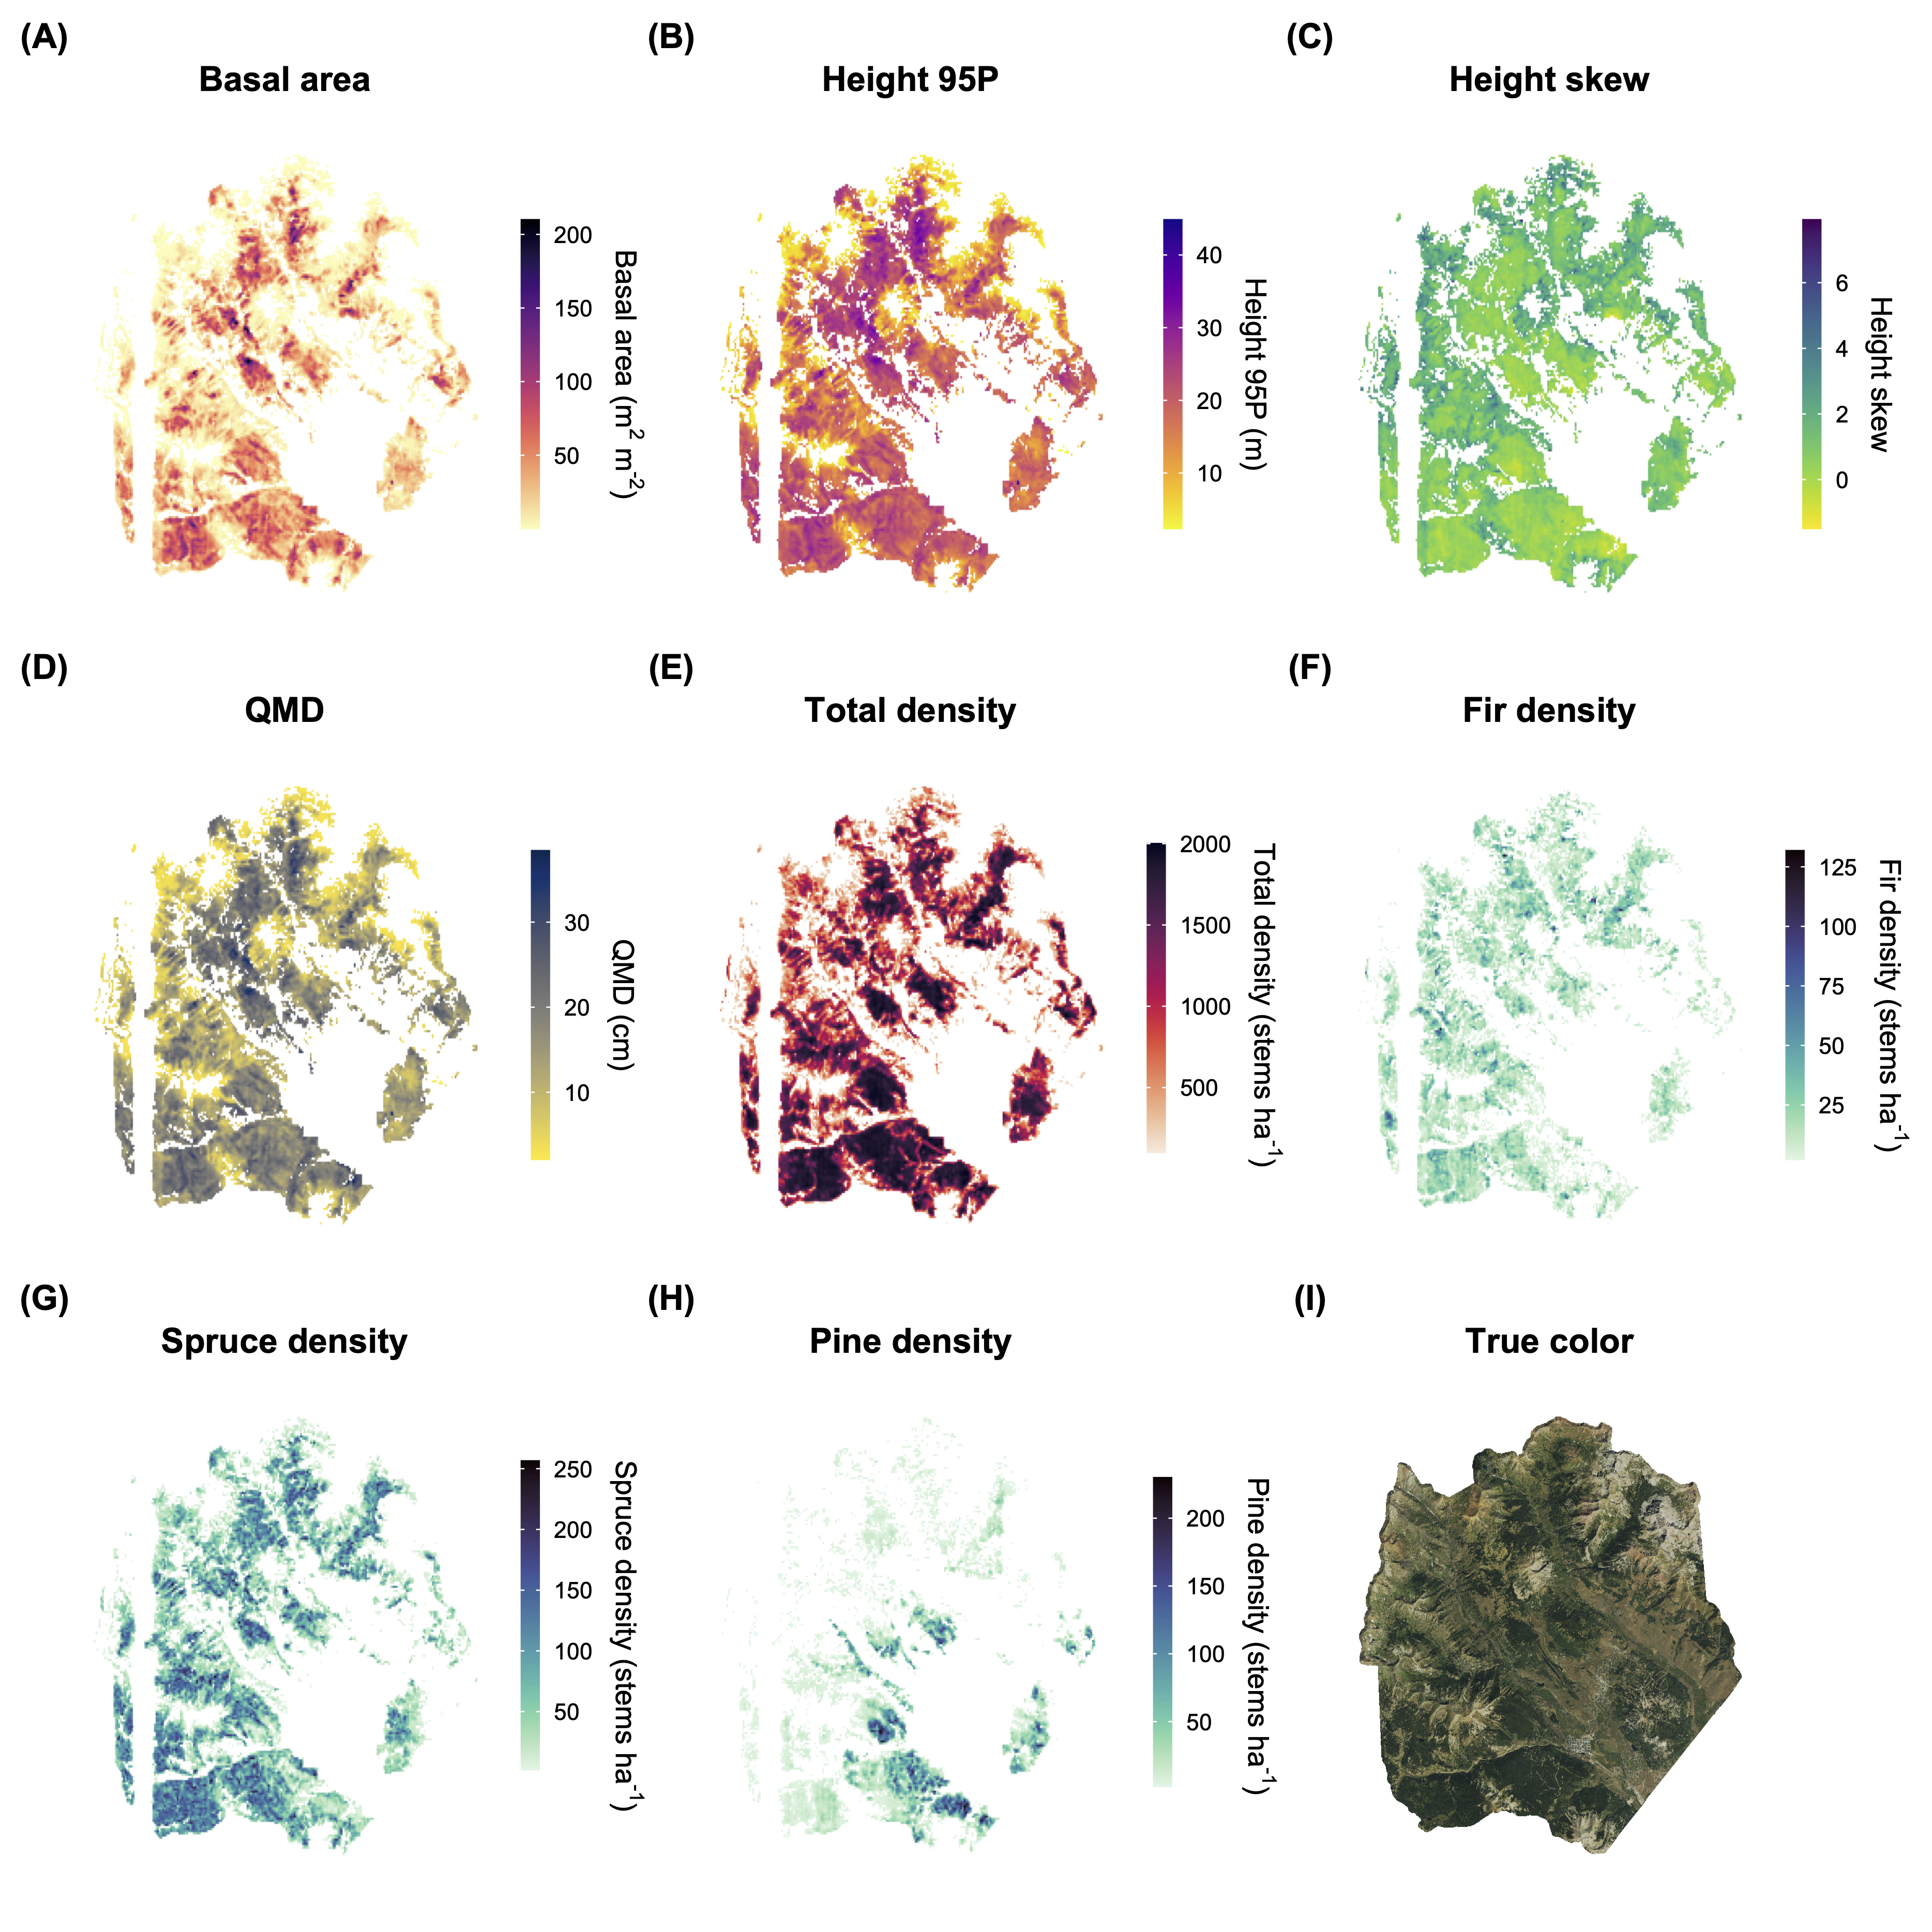
\includegraphics{./Figures/Fig5.png} \textbf{Figure 5.} Total number of
trees measured in plots (``Observed''---dark blue) and detected in
segmentation of the ALS point cloud (``Predicted''---light blue), by
height class, in 1 m increments. \clearpage

\newpage

\hypertarget{figure-6}{%
\subsection{Figure 6}\label{figure-6}}

\includegraphics{./Figures/Fig6.png} \textbf{Figure 6.} Variable
interaction plots demonstrate the strong, nonlinear elevational control
on density. Stand density was at a maximum at 3000 m, on ridgetops and
at southwest-facing aspects. \clearpage

\newpage

\hypertarget{table-3}{%
\subsection{Table 3}\label{table-3}}

\textbf{Table 3.} Response (RE) and explanatory (EX) variables used in
statistical analysis.

\begin{longtable}[]{@{}
  >{\raggedright\arraybackslash}p{(\columnwidth - 8\tabcolsep) * \real{0.12}}
  >{\raggedright\arraybackslash}p{(\columnwidth - 8\tabcolsep) * \real{0.24}}
  >{\raggedright\arraybackslash}p{(\columnwidth - 8\tabcolsep) * \real{0.32}}
  >{\raggedright\arraybackslash}p{(\columnwidth - 8\tabcolsep) * \real{0.15}}
  >{\raggedright\arraybackslash}p{(\columnwidth - 8\tabcolsep) * \real{0.18}}@{}}
\toprule
\begin{minipage}[b]{\linewidth}\raggedright
Type
\end{minipage} & \begin{minipage}[b]{\linewidth}\raggedright
Variable
\end{minipage} & \begin{minipage}[b]{\linewidth}\raggedright
Description
\end{minipage} & \begin{minipage}[b]{\linewidth}\raggedright
Units
\end{minipage} & \begin{minipage}[b]{\linewidth}\raggedright
Source
\end{minipage} \\
\midrule
\endhead
RE & Total number density & Total number of ITC objects per grid cell &
objects & NEON LiDAR \\
RE & Quadratic mean diameter & Quadratic mean of stem diameters of
objects per grid cell & cm & NEON LiDAR \\
RE & Basal area & Sum of cross-sectional areas of stems & m\(^2\) & NEON
LiDAR \\
RE & Above-ground biomass & Estimated ABG per grid cell & kg & NEON
LiDAR \\
RE & Height percentiles & 25th, 50th, 75th, and 90th percentile of
height per grid cell & m & NEON LiDAR \\
RE & Species composition & Basal area of each species as a proportion of
ground area per grid cell & unitless proportion & NEON LiDAR+
spectroscopy \\
RE & Species density & Number of stems of each species per grid cell &
stems / ha & NEON LiDAR \\
EX & Elevation & Elevation above sea level & m & NEON LiDAR \\
EX & Slope & dy/dx computed in a 30 m window & degrees & NEON LiDAR \\
EX & Folded aspect & Index of cardinal aspect adjusted for higher
incident radiation on SW slopes & unitless index & NEON LiDAR \\
EX & Heat load & Potential heat load calculated according to Eq. 3 in
McCune and Keon (2002) & unitless index & NEON LiDAR \\
EX & Topographic position index (1000 m) & Index of hillslope position
(summit, shoulder, backslope, footslope, and toeslope) computed in 1000
m window & unitless index & NEON LiDAR \\
EX & Topographic wetness index & Terrain-driven ratio of upslope water
supply to local drainage expressed as a function of local slope and
upslope contributing area per unit contour length, computed on a 100 m
pixel scale & unitless index & NEON LiDAR \\
EX & Soil available water capacity (AWC) & Amount of plant-available
water that can be stored in an increment of soil depth, inclusive of
fragments & SSURGO & \\
EX & Soil organic matter (OM) & Amount of decomposed plant and animal
residue expressed as a weight percentage of the less than 2 mm soil
material & weight \% & SSURGO \\
EX & Soil \(k_{sat}\) & Amount of water that would move vertically
through a unit area of saturated soil per unit time under unit hydraulic
gradient & \(\mu m/sec\) {[}TODO: confirm{]} & SSURGO \\
EX & Soil total depth & Sum of horizon depths in a component & cm &
SSURGO \\
EX & Snow water equivalent (SWE) & Snow water equivalent derived by
forcing iSnobal with 50 m snow depth data from eight Airborne Snow
Observatory flights & ASO & \\
EX & Lithologic substrate & Distribution of rock formations & Colorado
Geological Survey & \\
\bottomrule
\end{longtable}

\clearpage

\newpage

\hypertarget{figure-7}{%
\subsection{Figure 7}\label{figure-7}}

\includegraphics{./Figures/Fig7.png} \textbf{Figure 7.} Stand density
increased with soil organic matter and was at minimum with soil total
depth = 50 cm, but other soil properties had little correlation with
stand density. \clearpage

\newpage

\hypertarget{figure-8}{%
\subsection{Figure 8}\label{figure-8}}

\includegraphics{./Figures/Fig8.png} \textbf{Figure 8.} Snow-water
equivalent (SWE) mediated the elevational control on density, 90th
percentile height, and quadratic mean diameter. SWE has an overall
flattening effect on the elevation-density curve. Where SWE is high and
elevation is high, density is also at a maximum. Where SWE is high but
elevation is low, this has a substantial dampening effect on all three
structural parameters. \clearpage

\newpage

\hypertarget{figure-9}{%
\subsection{Figure 9}\label{figure-9}}

\includegraphics{./Figures/Fig9.png} \textbf{Figure 9.} Elevation
accounted for differences in the shape of allometric curves describing
the relationship between tree DBH and height. Curves are fitted to
census data according to the function height = A(DBHb) (A). The
coefficient A in the equation declines with elevation, indicating that,
as elevation increases, height growth diminishes per unit growth in
girth (B).

\clearpage

\hypertarget{supplementary-materials}{%
\section{Supplementary Materials}\label{supplementary-materials}}

\hypertarget{references}{%
\section*{References}\label{references}}
\addcontentsline{toc}{section}{References}

\hypertarget{refs}{}
\begin{CSLReferences}{1}{0}
\leavevmode\vadjust pre{\hypertarget{ref-amundson_state_1997}{}}%
Amundson, R., Jenny, H., 1997. On a {State} {Factor} {Model} of
{Ecosystems}. BioScience 47, 536--543.
\url{https://doi.org/10.2307/1313122}

\leavevmode\vadjust pre{\hypertarget{ref-bolstad_forests_2018}{}}%
Bolstad, P.V., Elliott, K.J., Miniat, C.F., 2018. Forests, shrubs, and
terrain: Top‐down and bottom‐up controls on forest structure. Ecosphere
9. \url{https://doi.org/10.1002/ecs2.2185}

\leavevmode\vadjust pre{\hypertarget{ref-dalponte_tree-centric_2016}{}}%
Dalponte, M., Coomes, D.A., 2016. Tree-centric mapping of forest carbon
density from airborne laser scanning and hyperspectral data. Methods in
Ecology and Evolution 7, 1236--1245.
\url{https://doi.org/10.1111/2041-210X.12575}

\leavevmode\vadjust pre{\hypertarget{ref-jenny_derivation_1961}{}}%
Jenny, H., 1961. Derivation of {State} {Factor} {Equations} of {Soils}
and {Ecosystems}. Soil Science Society of America Journal 25, 385--388.
\url{https://doi.org/10.2136/sssaj1961.03615995002500050023x}

\leavevmode\vadjust pre{\hypertarget{ref-kane_water_2015}{}}%
Kane, V.R., Lutz, J.A., Alina Cansler, C., Povak, N.A., Churchill, D.J.,
Smith, D.F., Kane, J.T., North, M.P., 2015. Water balance and topography
predict fire and forest structure patterns. Forest Ecology and
Management 338, 1--13.
\url{https://doi.org/10.1016/j.foreco.2014.10.038}

\leavevmode\vadjust pre{\hypertarget{ref-lookingbill_empirical_2004}{}}%
Lookingbill, T., Urban, D., 2004. An empirical approach towards improved
spatial estimates of soil moisture for vegetation analysis. Landscape
Ecology 19, 417--433.
\url{https://doi.org/10.1023/B:LAND.0000030451.29571.8b}

\leavevmode\vadjust pre{\hypertarget{ref-lydersen_topographic_2012}{}}%
Lydersen, J., North, M., 2012. Topographic {Variation} in {Structure} of
{Mixed}-{Conifer} {Forests} {Under} an {Active}-{Fire} {Regime}.
Ecosystems 15, 1134--1146.
\url{https://doi.org/10.1007/s10021-012-9573-8}

\leavevmode\vadjust pre{\hypertarget{ref-mcnab_topographic_1993}{}}%
McNab, W.H., 1993. A topographic index to quantify the effect of
mesoscale landform on site productivity. Canadian Journal of Forest
Research 23, 1100--1107. \url{https://doi.org/10.1139/x93-140}

\leavevmode\vadjust pre{\hypertarget{ref-mcnab_terrain_1989}{}}%
McNab, W.H., 1989. Terrain {Shape} {Index}: {Quantifying} {Effect} of
{Minor} {Landforms} on {Tree} {Height}. Forest Science 35, 91--104.
\url{https://doi.org/10.1093/forestscience/35.1.91}

\end{CSLReferences}

\end{document}
